\documentclass[a4paper,11pt,final]{report}
\usepackage[utf8]{inputenc} % Prendre en compte les caractères accentués
\usepackage[francais]{babel} % Prendre en compte les particularités de la typographie française.
\usepackage{geometry}         % marges
\usepackage{graphicx}         % images
\usepackage{setspace}
\usepackage[french]{varioref}
\usepackage{titlesec}  %titlespacing
\usepackage{caption}

\titlespacing{\chapter}{0pt}{*-5}{*5}
\titlespacing{\section}{0pt}{*2}{*2}
\titleformat{\chapter}[hang]{\bf\huge}{\thechapter}{2pc}{}
%\titleformat{\chapter}[hang]{\bf\huge}{\thechapter}{14pt}{\LARGE}
\renewcommand{\baselinestretch}{1.2}
\setlength{\parskip}{1.5ex plus .4ex minus .4ex}
\setlength{\parindent}{15pt} 
%\setlength{\topmargin}{-35pt}
%\setlength{\textheight}{600pt}


\title{\textbf{Manuel d'utilisation}\\UniForms}
\author{}
\date{}
\begin{document}

\maketitle
\setcounter{page}{2}
\tableofcontents 
%Se mettre au niveau d'un non informaticien
%Expliquer les enchainements de fenêtre, erreurs
%FAQ
\chapter{Généralités}
\section{But de l'application}
Uniforms a pour but de fournir une plateforme de gestion de formulaires. C'est-à-dire, proposer des fonctionnalités de création et de soumission de formulaires ainsi que la possibilité de répondre à ces derniers et de consulter les réponses par le créateur du formulaire.

\section{Public visé}
Ce manuel est destiné aux personnes désirant créer un formulaire, le soumettre à une ou plusieurs personnes et consulter les réponses faites par les destinataires, mais aussi aux personnes répondant aux formulaires envoyés par l'intermédiaire de la plateforme uniforms.

\section{Installation}
Une fois les fichiers sources sur le serveur, aller sur la page res/sql/Installer.php figure~\ref{install} plusieurs informations vous serons demandées, le serveur, le nom d'utilisateur, le mot de passe et le nom de la base de données.

\noindent\begin{minipage}{\linewidth}% to keep image and caption on one page
\makebox[\linewidth]{%        to center the image
  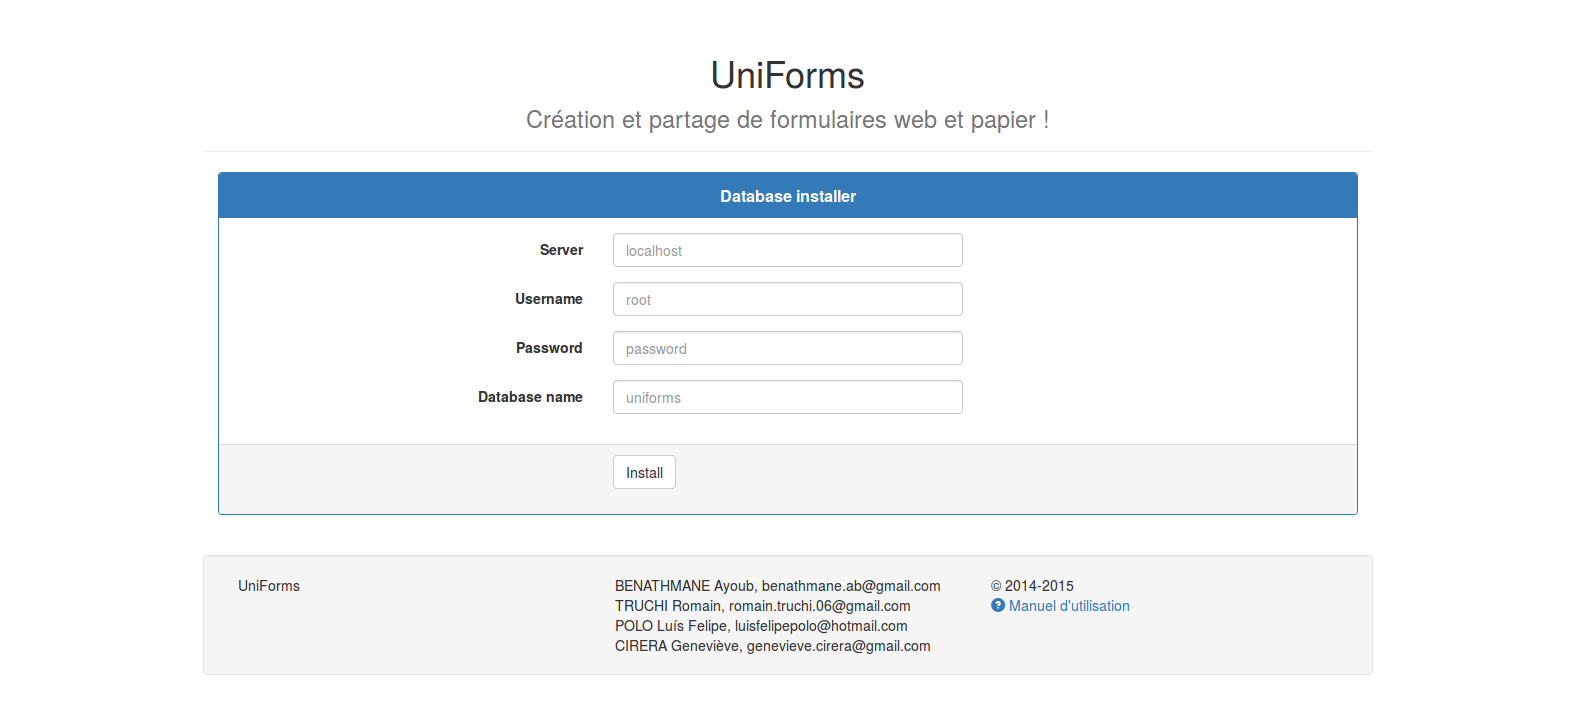
\includegraphics [width=180mm]{images/installer.png}}
\captionof{figure}{Page d'installation}\label{install}
\end{minipage}

\chapter{Fenêtre principale}
\section{Authentification}
La première page affichée est celle de l'authentification, que l'on peut voir figure~\ref{authentificationChoix}, elle en propose deux types : CAS (pour les utilisateurs disposants d'un identificant CAS commençant par les initiales du nom et prénom puis du numéro étudiant) ou autres utilisateurs.\\
%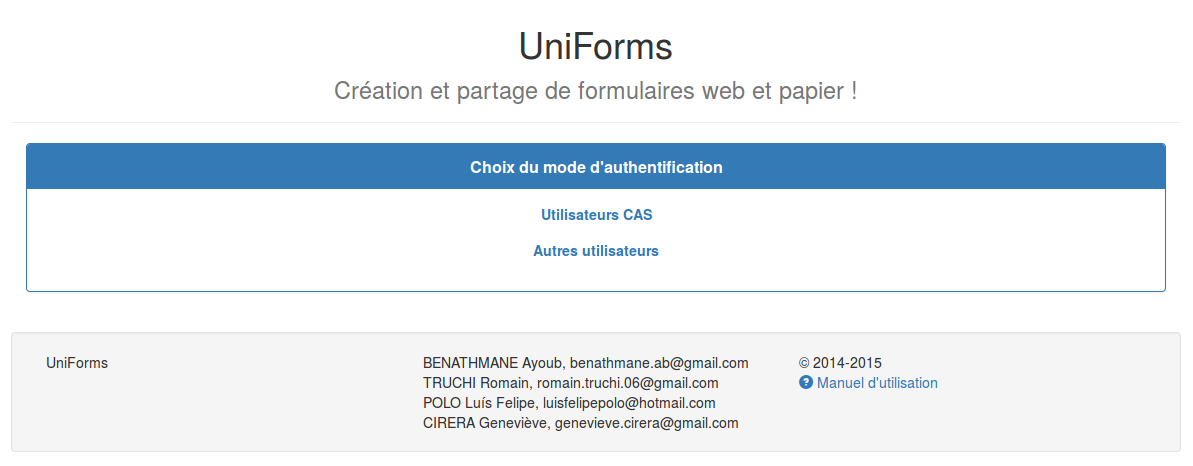
\includegraphics[width=.7\paperwidth]{images/authentification.png}\label{fig:ArgSimple}
\noindent\begin{minipage}{\linewidth}% to keep image and caption on one page
\makebox[\linewidth]{%        to center the image
  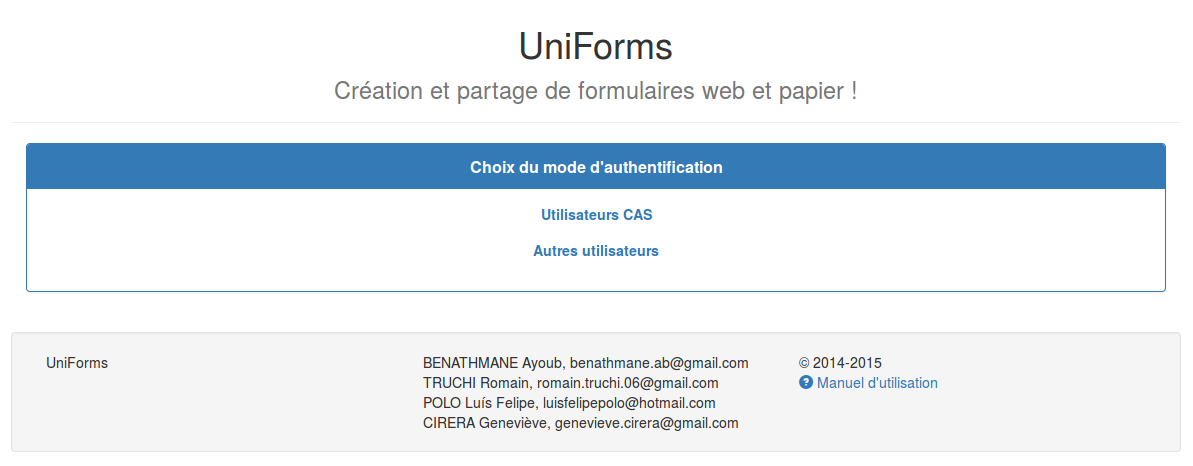
\includegraphics [width=150mm]{images/authentification.png}}
\captionof{figure}{Page de choix d'authentification}\label{authentificationChoix}
\end{minipage}

Pour accéder à la page d'authentification, il suffit de cliquer sur ``Utilisateurs CAS'' ou ``Autres utilisateurs''
\subsection{Utilisateur CAS}
Une fois choisi l'authentification CAS, la page figure~\ref{authentificationCAS} s'affiche.\\
Dans le champs ``Identification'', mettre votre identifiant (ex : dj209832, pour Jean Dupont ayant pour numéro étudiant 209832).\\
Entrer le mot de passe puis cliquer sur ``SE CONNECTER''. Si l'authentification échoue, une alerte ``Mauvais identifiant / mot de passe'' apparaitra pour vous en informer. Si elle réussit, la page d'accueil, figure~\ref{pageAccueil}, s'affichera. 

\noindent\begin{minipage}{\linewidth}% to keep image and caption on one page
\makebox[\linewidth]{%        to center the image
  
\includegraphics [width=150mm]{images/authCAS.png}}
\captionof{figure}{Authentification CAS}\label{authentificationCAS}
\end{minipage}

\subsection{Autres utilisateurs}
Si vous possédez un compte, cliquer sur ``Autre utilisateurs'' affichera la page figure~\ref{authentificationAutre}. Entrez votre identifiant et mot de passe, cliquez ensuite sur ``Connection''.\\
Si l'authentification réussi vous accederez à la page d'accueil figure~\ref{pageAccueil}, si elle échoue, vous serez redirigé vers la page de connection figure~\ref{authentificationChoix}

\noindent\begin{minipage}{\linewidth}% to keep image and caption on one page
\makebox[\linewidth]{%        to center the image
  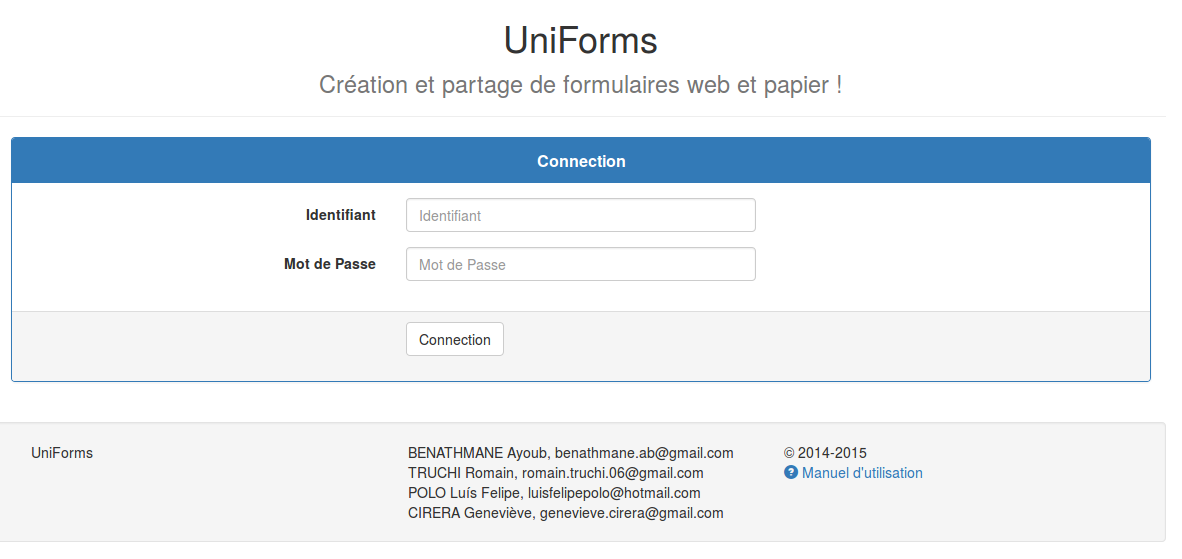
\includegraphics [width=150mm]{images/authentificationAutre.png}}
\captionof{figure}{Authentification autre utilisateur}\label{authentificationAutre}
\end{minipage}

\section{Page d'accueil}
Après authentification, la page figure~\ref{pageAccueil} s'affiche. On peut noter trois zones principales, une barre d'option, une zone des trois derniers formulaires créés et une zone avec les trois derniers formulaires à répondre ou répondus.\\
\noindent\begin{minipage}{\linewidth}% to keep image and caption on one page
\makebox[\linewidth]{%        to center the image
  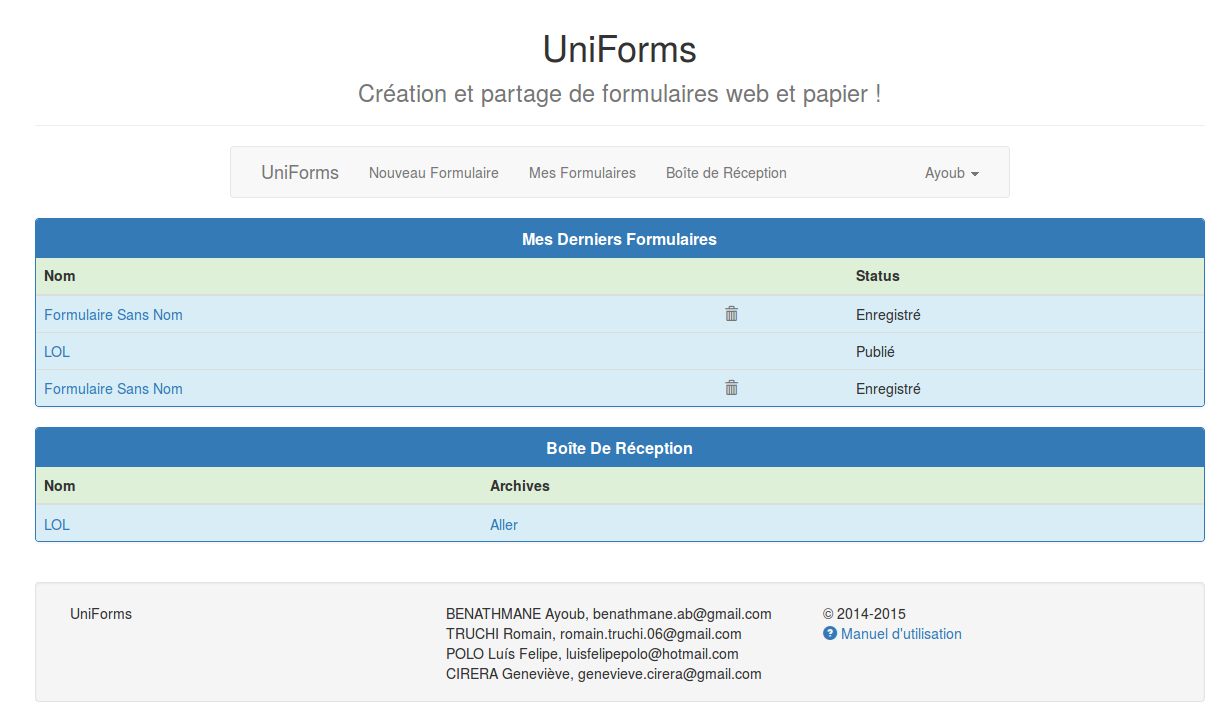
\includegraphics [width=160mm]{images/pageAccueil.png}}
\captionof{figure}{Page d'accueil}\label{pageAccueil}
\end{minipage}

\subsection{La barre d'options}\label{sec:barreOption}
La barre d'options figure~\ref{barreOptions} propose divers boutons : ``Uniforms'', ``Nouveau Formulaire'', ``Mes Formulaires'', ``Boite de Réception'' et ``Ayoub''. Les actions au clique de ces boutons sont les suivantes :
\begin{description}
	\item [Uniforms] : Retour à la page d'accueil figure~\ref{pageAccueil}
	\item [Nouveau Formulaire] : Redirection vers la page de création d'un nouveau formulaire figure~\ref{pageCreation}
	\item [Mes Formulaires] : Redirection vers les formulaires que vous avez créés figure~\ref{zoneFormCree}.
	\item [Boite de Réception] : Redirige vers la page où se situe la liste de tous les formulaires auxquels vous pouvez répondre figure~\ref{zoneFormRecu} ou avez répondu.
	\item [Ayoub] : Identifiant de la personne dont la session est ouverte, au clique, l'option ``Logout'' s'affiche pour la déconnection.
\end{description}

\noindent\begin{minipage}{\linewidth}% to keep image and caption on one page
\makebox[\linewidth]{%        to center the image
  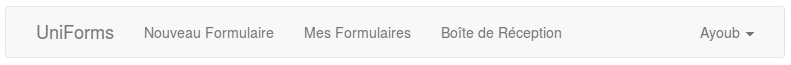
\includegraphics [width=140mm]{images/barreOptions.png}}
\captionof{figure}{Barre d'options}\label{barreOptions}
\end{minipage}

\subsection{Zone ``Mes Formulaires''}
Cette zone est présente sur la page d'accueil (avec les trois derniers) et sur la page de ``Mes Formulaires'' figure~\ref{zoneFormCree}. La zone de formulaires créés liste l'ensemble des formulaires créés par l'utilisateur courant, les validés et non validés, figure~\ref{zoneFormCree}.\\
Un formulaire non validé peut être supprimé en cliquant sur la corbeille de la deuxième colonne.\\
Sur la colonne ``Status'', l'état du formulaire est affiché, ``Enregistré'' ou ``Publié''.

\noindent\begin{minipage}{\linewidth}% to keep image and caption on one page
\makebox[\linewidth]{%        to center the image
  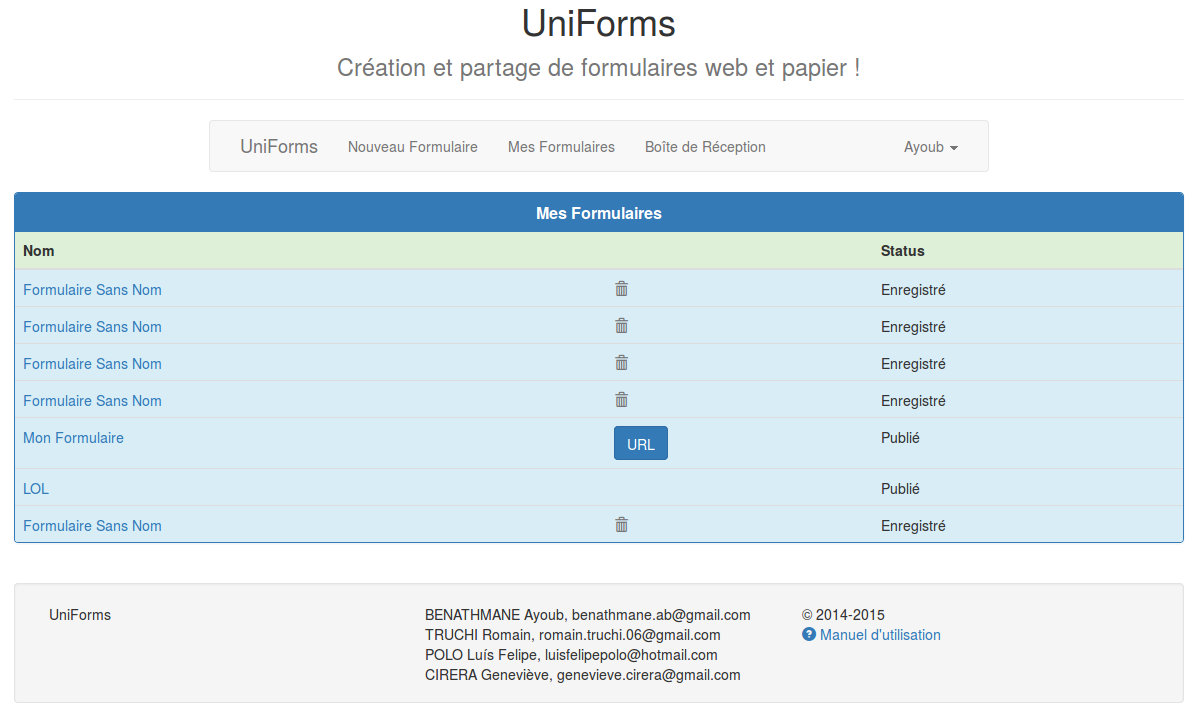
\includegraphics [width=140mm]{images/pageMesFormulaires.png}}
\captionof{figure}{Liste des formulaires créés}\label{zoneFormCree}
\end{minipage}

\subsubsection{Les formulaires validés}
Les formulaires validés ne peuvent plus être modifiés, ils ont été envoyés aux destinataires. La seule action possible sur ces formulaires est voir les résultats en cliquant sur le nom du formulaire souhaité qui montre les réponses du formulaire qui ont déjà été faites par les destinataires.\\
Si le formulaire est anonyme, on peut obtenir l'url en cliquant sur le bouton ``URL'' figure~\ref{urlForm} de ce formulaire afin de l'envoyer par mail à un destinataire.

\noindent\begin{minipage}{\linewidth}% to keep image and caption on one page
\makebox[\linewidth]{%        to center the image
  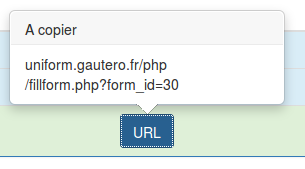
\includegraphics [width=50mm]{images/urlForm.png}}
\captionof{figure}{URL d'un formulaire validé}\label{urlForm}
\end{minipage}

\subsubsection{Les formulaires non validés}
Les formulaires non validés n'ont pas encore été envoyés aux destinataires, ils peuvent donc être modifiés en cliquant sur le nom du formulaire souhaité. Cette action mènera à la page de création figure~\ref{pageCreation} pré-rempli par les éléments enregistrés.

\subsection{Zone ``Boite de reception''}
Dans cette zone figure~\ref{zoneFormRecu} est listé l'ensemble des formulaires dont l'utilisateur courant est destinataire, c'est-à-dire ceux pour lesquels il doit répondre ou doit répondre.\\

\noindent\begin{minipage}{\linewidth}% to keep image and caption on one page
\makebox[\linewidth]{%        to center the image
  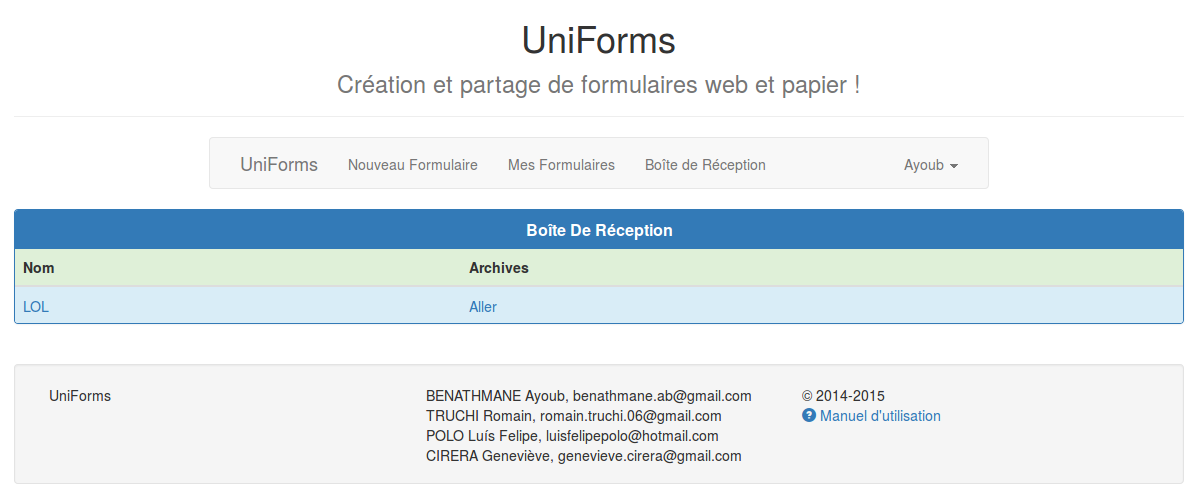
\includegraphics [width=150mm]{images/pageBoiteRecep.png}}
\captionof{figure}{Zone de formualaires reçus}\label{zoneFormRecu}
\end{minipage}

En cliquant sur le nom du formulaire, vous êtes redirigés vers une page qui liste toutes les réponses initiées pour ce formulaire.\\
Plusieurs cas peuvent se produire :
\begin{itemize}
	\item Vous avez épuisé le nombre de réponse autorisée, vous ne pouvez donc plus répondre. figure~\ref{listRepNone}
	
\noindent\begin{minipage}{\linewidth}% to keep image and caption on one page
\makebox[\linewidth]{%        to center the image
  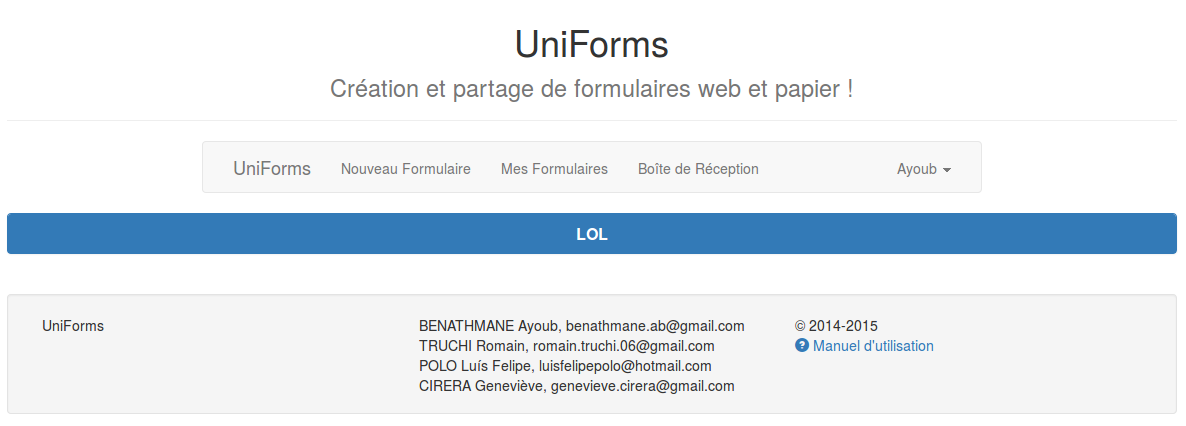
\includegraphics [width=150mm]{images/listRepNone.png}}
\captionof{figure}{Liste des réponses du formulaire ``LOL''}\label{listRepNone}
\end{minipage}

	\item Le formulaire ne se rempli que par vous et il vous reste des réponses à effectuer figure~\ref{listRepMulti}. Ici, ``Ayoub'' est la personne vous ayant soumis le formulaire, entre parenthèses est indiqué le nombre de réponses restantes en plus de celle commencée indiquée par ``Réponse \#0''.\\
	La réponses initiée ``Réponse \#0'' peut être modifié en cliquant sur son lien, la page de réponses figure~\ref{repondre} s'affiche pré-remplie.\\
	Cliquer sur ``Nouvelle réponse'', initialisera une nouvelle réponse en vous redirigeant vers la page de réponse figure~\ref{repondre}.
	
	\noindent\begin{minipage}{\linewidth}% to keep image and caption on one page
\makebox[\linewidth]{%        to center the image
  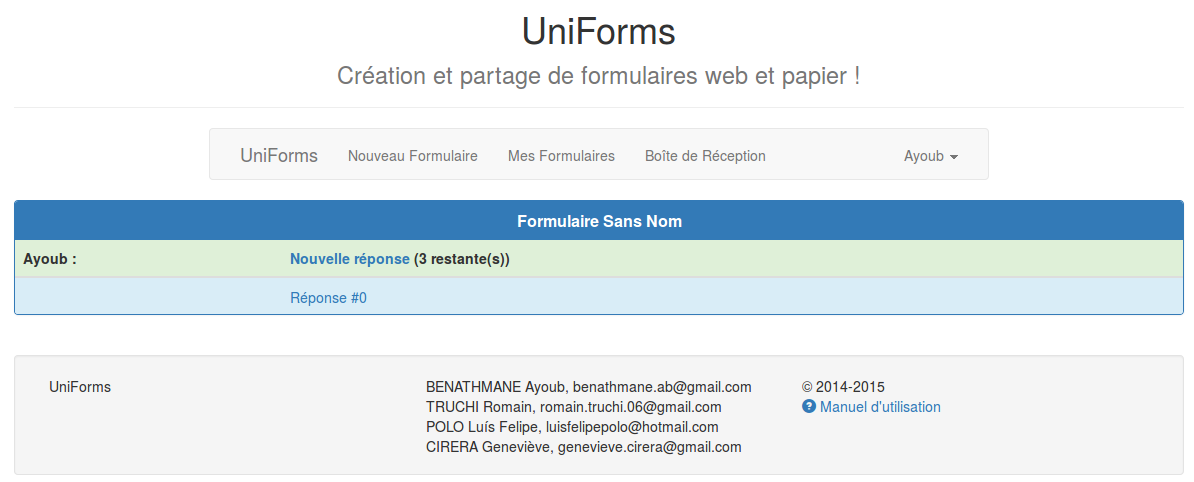
\includegraphics [width=150mm]{images/listRepMulti.png}}
\captionof{figure}{Liste des réponses du formulaire ``Formulaire Sans Nom''}\label{listRepMulti}
\end{minipage}

	\item Le formulaire se rempli à plusieurs et vous quelqu'un a déjà répondu avant vous. Dans ce cas, figure~\ref{listRepMultiGroup} on peut voir deux lignes car le formulaire a été soumis par ``Ayoub'' avec un nombre maximum de réponse supérieur ou égal à deux. Geneviève a répondu 2 fois à ce même formulaire, maintenant c'est votre tour de répondre, et vous ne pouvez répondre qu'une seule fois pour chaque formulaire vous ayant parvenu (nombre indiqué entre parenthèses).
	
	\noindent\begin{minipage}{\linewidth}% to keep image and caption on one page
\makebox[\linewidth]{%        to center the image
  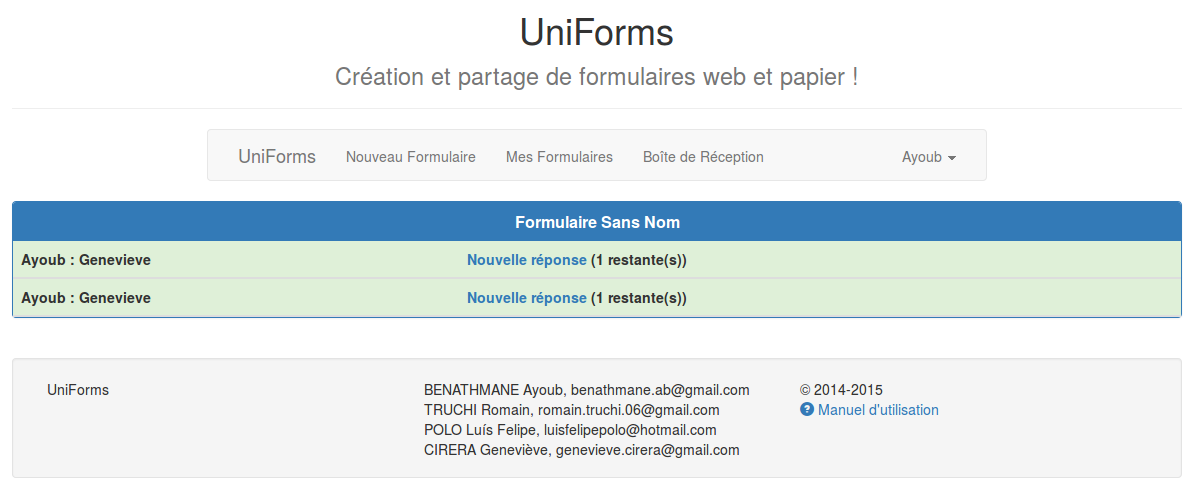
\includegraphics [width=150mm]{images/listRepMultiCollab.png}}
\captionof{figure}{Liste des réponses du formulaire ``Formulaire Sans Nom'' ayant été répondu par une autre personne également}\label{listRepMultiGroup}
\end{minipage}
\end{itemize}

En cliquant sur ``Aller'' figure~\ref{zoneFormRecu}, vous accédez à la liste de toutes les réponses que vous avez envoyé pour ce formulaire. Figure~\ref{consultRepEnvoye} on peut voir que vous avez envoyé 2 réponses pour un formulaire soumis par ``Ayoub'' et répondu ensuite par ``Geneviève''. Vous pouvez ensuite consulter ce que vous avez répondu en cliquant sur les liens ``Réponse\#0''. Si plus d'une réponse a été envoyé, il y aura ``Réponse\#0'', ``Réponse\#1'',...

\noindent\begin{minipage}{\linewidth}% to keep image and caption on one page
\makebox[\linewidth]{%        to center the image
  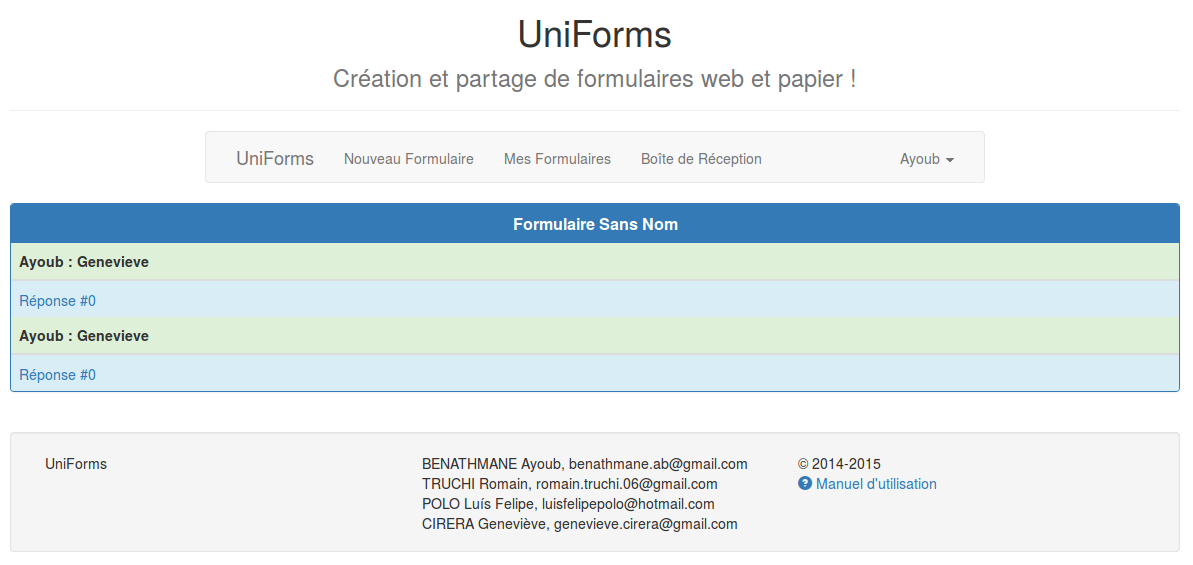
\includegraphics [width=150mm]{images/consultRepEnvoye.png}}
\captionof{figure}{Liste des réponses envoyées pour le formulaire ``Formulaire Sans Nom''}\label{consultRepEnvoye}
\end{minipage}

\chapter{Création}
\section{Créer un formulaire}\label{CreerFormulaire}
Pour créer un formulaire, la première étape est de cliquer sur le bouton ``Nouveau Formulaire'' de la barre d'options, voir figure~\ref{barreOptions}. Ensuite la page de création, figure~\ref{pageCreation}, s'affiche.\\
On peut distinguer plusieurs zones. On retrouve tout d'abord la barre d'option vu section~\ref{sec:barreOption}, puis une zone de ``Groupe'' à gauche, une zone avec une page quadrillée puis sur le coté droit, deux petites zones, une avec deux cases à cocher figure~\ref{params} et une autre avec une liste d'élément figure~\ref{elements}.\\
Tout en bas de cette page, deux boutons ``Enregistrer'' et ``Publier'', permettant respectivement d'enregistrer un formulaire (afin de pouvoir le modifier par la suite) et de publier un formulaire, ce dernier sera alors envoyé aux destinataires, aucune modification ne sera alors permise.

\noindent\begin{minipage}{\linewidth}% to keep image and caption on one page
\makebox[\linewidth]{%        to center the image
  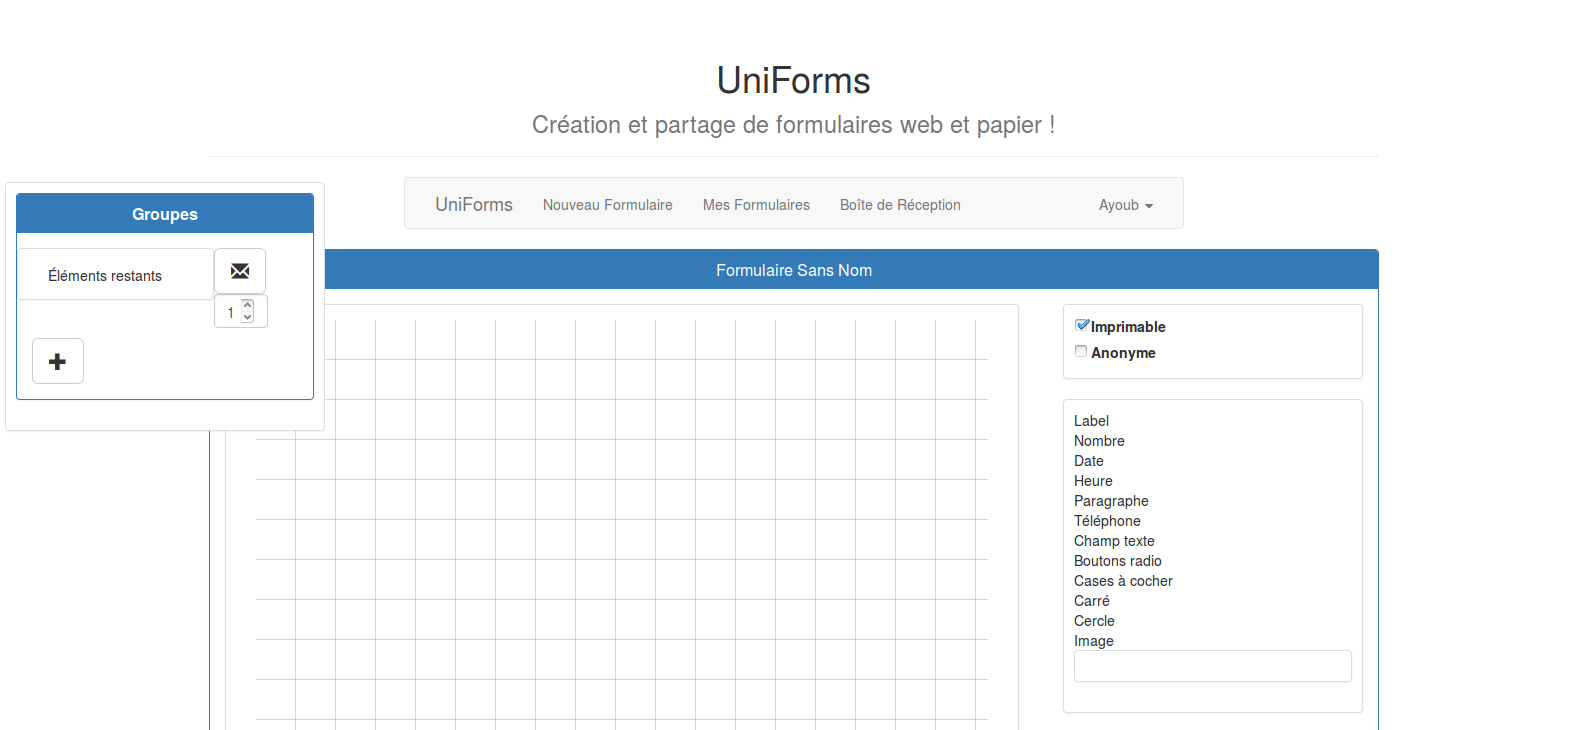
\includegraphics [width=150mm]{images/pageCreation.png}}
\captionof{figure}{Page de création de formulaire}\label{pageCreation}
\end{minipage}

\subsection{Zone de ``Paramètres''}
Deux champs sont paramètrables, figure~\ref{parametreCreation} :
\begin{description}
	\item [Imprimable] : à cocher si vous souhaitez imprimer le formulaire
	\item [Anonyme] : à cocher si vous ne souhaitez pas définir de destinataire en particulier. Ce formulaire sera donc en accès libre à toutes les personnes disposants de son lien url.
	%\item [Nombre de réponses max] : Vous pouvez définir le nombre de réponse possible pour le formulaire. Si vous mettez ``3'', chaque destinataire pourra répondre trois fois à ce même formulaire. Si vous souhaitez que le nombre de réponses soit infini, mettez ``0''.
\end{description}

\noindent\begin{minipage}{\linewidth}% to keep image and caption on one page
\makebox[\linewidth]{%        to center the image
  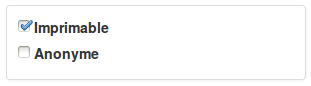
\includegraphics [width=50mm]{images/params.png}}
\captionof{figure}{Paramètres de création de formulaire}\label{parametreCreation}
\end{minipage}

\subsection{Zone de ``Groupe''}
Cette zone figure~\ref{zoneGroup} permet de créer des groupes d'éléments et de les assigner à une ou plusieurs personnes. Elle permet notamment de créer un formulaire pour une demande d'autorisation soumis à plusieurs personnes et ayant la même personne pour sa validation.\\
Le groupe ``Éléments restants'' n'est pas supprimable, il contient par défaut tous les éléments n'appartenant à aucun autre groupe.\\

\noindent\begin{minipage}{\linewidth}% to keep image and caption on one page
\makebox[\linewidth]{%        to center the image
  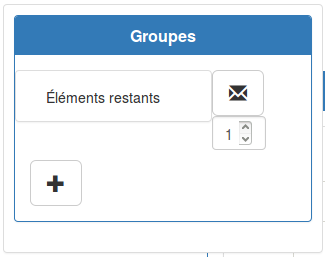
\includegraphics [width=60mm]{images/zoneGroup.png}}
\captionof{figure}{Zone de groupes}\label{zoneGroup}
\end{minipage}

Pour ajouter des groupes, cliquer sur le bouton ``+'', ensuite glissez-déposez les éléments que vous souhaitez mettre dans ce groupe.\\
Pour assigner des destinataires à un groupe, cliquez sur la bouton avec l'enveloppe une fenêtre modale figure~\ref{modaleDest} s'ouvrira.
Le nombre en dessous du bouton avec l'enveloppe correspond au nombre de réponse maximum autorisé au(x) destinataire(s) de ce groupe.

\subsection{Destinataires}
Pour sélectionner un destinataire, ouvrez la fenêtre modale figure~\ref{modaleDest}, commencez à écrire son numéro étudiant ou identifiant dans le champs d'entrée, une liste déroulante apparaitra avec toutes les possibilités. 

\noindent\begin{minipage}{\linewidth}% to keep image and caption on one page
\makebox[\linewidth]{%        to center the image
  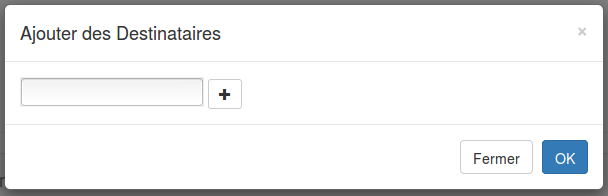
\includegraphics [width=80mm]{images/modaleDest.png}}
\captionof{figure}{Fenêtre modale pour la sélection des destinataires}\label{destinatairesCheckbox}
\end{minipage}

Sélectionnez ensuite le destinataire souhaité et cliquez sur ``+'', le destinataire s'affichera alors à coté avec une checkbox figure~\ref{destinatairesCheckbox}. Si vous souhaitez éliminer un destinataire, décochez la checkbox.


\noindent\begin{minipage}{\linewidth}% to keep image and caption on one page
\makebox[\linewidth]{%        to center the image
  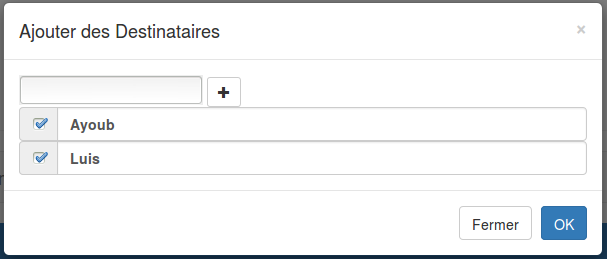
\includegraphics [width=80mm]{images/modalDestCheckbox.png}}
\captionof{figure}{Fenêtre modale pour la sélection des destinataires avec deux destinataires sélectionnés}\label{zoneGroup}
\end{minipage}

\subsection{Éléments}
Douze éléments sont disponibles, figure~\ref{elements}, pour les utiliser il suffit de les glisser-déposer avec la souris sur la page quadrillée. Vous trouverez en annexe, le descriptif de chaque élément.

\noindent\begin{minipage}{\linewidth}% to keep image and caption on one page
\makebox[\linewidth]{%        to center the image
  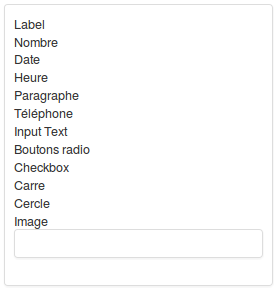
\includegraphics [width=60mm]{images/elements.png}}
\captionof{figure}{Éléments disponibles pour la création}\label{elements}
\end{minipage}

\subsubsection{Ajouter un élément}
Pour ajouter un élément, le placer par glisser-déposer\footnote{Aussi appelé Drag and drop : maintenir appuyer sur l'élément et déplacer la souris jusqu'à la zone choisie, relacher la pression} sur la zone quadrillée.\\ 
L'élément est ensuite paramétrable par une série de champs s'affichant en dessous de la liste des éléments personnels à chaque type d'élément.
Si un élément est placé à l'extérieur de la zone autorisé, il reviendra à sa place d'origine.

\subsubsection{Modifier un élément}
Pour modifier un élément, cliquer sur celui-ci, il s'encadre alors en rouge et les champs de paramétrage s'affiche à droite. Modifier les valeurs souhaitées. La taille hauteur et largeur peuvent également être modifiées par la souris. Par survol de la souris, une flèche apparait en bas à droite de l'élément, elle permet le redimensionnement de l'élément.\\
Vous pouvez également déplacer l'élément par un simple glisser-déposer à l'intérieur de la zone quadrillée.

\subsubsection{Supprimer un élément}
Pour supprimer un élément, il suffit de sélectionner l'élément, il doit apparaitre encadré en rouge, puis de presser la touche ``Del'' ou ``Suppr''.

\subsection{Page quadrillée}
La page quadrillée est la zone du formulaire, les éléments y sont placés. La hauteur et la largeur de cette zone est celle d'une page A4, la délimitation entre deux pages différentes est marquée par un trait noir horizontal.\\
Lors de l'ajout d'éléments, si un élément est placé bas dans la page, la zone s'aggrandit automatiquement de la hauteur d'une page A4. 

\section{Modifier un formulaire}
Pour modifier un formulaire, il faut tout d'abord cliquer sur le nom du formulaire que l'on souhaite modifier sur la page de ``Mes Formulaires'' figure~\ref{zoneFormCree}, ce qui ouvrira la page de création de formulaire vue section~\ref{CreerFormulaire}. Cette page est remplie par les éléments, destinataires et paramètres enregistrés précédemment. Vous pouvez alors modifier ce que vous souhaitez, le ré-enregistrer ou le valider.

\section{Consulter les réponses d'un formulaire}
Sur la page ``Mes Formulaires'' figure~\ref{zoneFormCree}, cliquer sur le nom d'un formulaire publié amène à la page où se situe toute la liste des réponses qui ont été effectuée figure~\ref{consultResult}.
%En ligne, il suffit de cliquer sur les liens ``Réponse \#0'', ``Réponse \#1'',... ce qui affiche les formulaires remplis figure~\ref{consultResultForm}.

\noindent\begin{minipage}{\linewidth}% to keep image and caption on one page
\makebox[\linewidth]{%        to center the image
  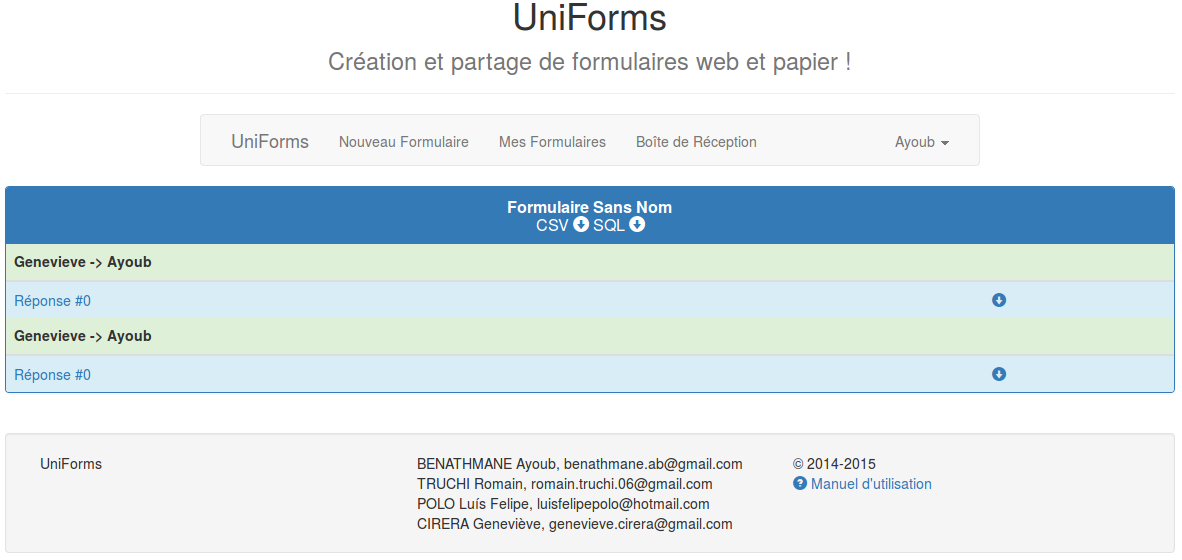
\includegraphics [width=150mm]{images/listReponseConsultation.png}}
\captionof{figure}{Page de consultation des réponses}\label{consultResult}
\end{minipage}

Ici, vous avez la possibilité de consulter les réponses sous deux formes, directement sous la forme du formulaire rempli en cliquant sur ``Réponse \#0'', ``Réponse \#1'',..., cela vous mène à la page figure~\ref{consultResultForm}. Ou bien, en téléchargeant le fichier CSV par réponse en cliquant sur l'icone de la colonne de droite ou en cliquant sur les icone de CSV ou SQL pour respectivement télécharger tous les résults en CSV et SQL.\\
Sur la page figure~\ref{consultResultForm}, vous avez la possibilité de passer de résultats en résultats grâce aux boutons ``Previous'' et ``Next'', le bouton ``Back'' vous ramène à la page figure~\ref{consultResult}.

\noindent\begin{minipage}{\linewidth}% to keep image and caption on one page
\makebox[\linewidth]{%        to center the image
  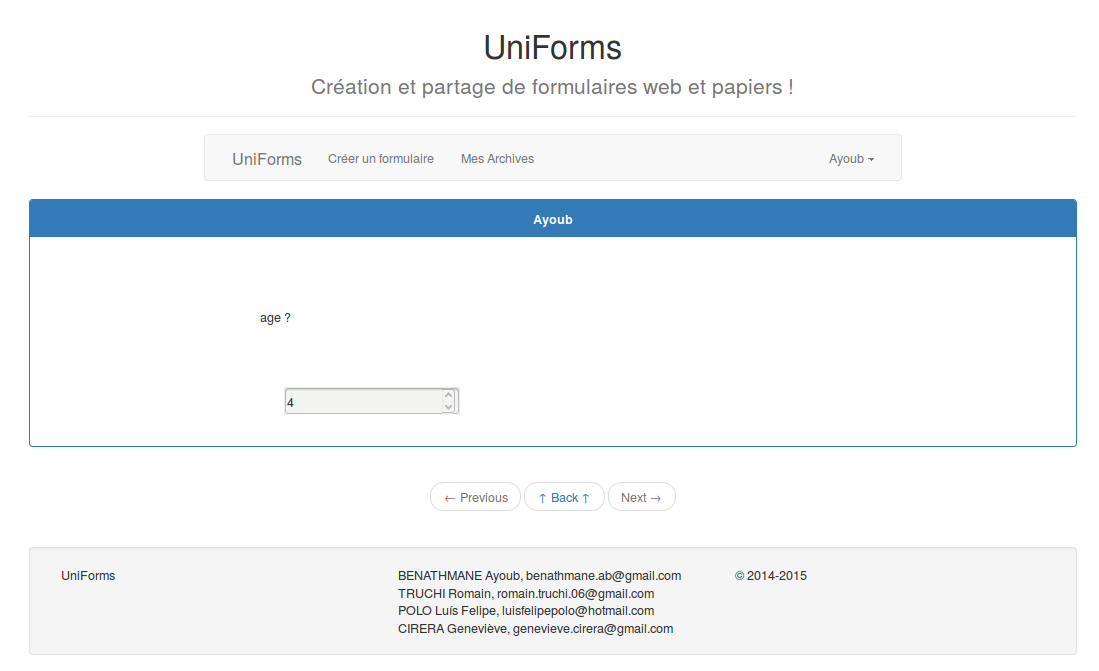
\includegraphics [width=150mm]{images/consultResultForm.png}}
\captionof{figure}{Formulaire rempli par un destinataire}\label{consultResultForm}
\end{minipage}


\chapter{Répondre}
\section{Répondre à un formulaire}
Pour répondre à un formulaire, il suffit de cliquer sur ``Nouvelle réponse'' figure~\ref{zoneFormRecu}. La page de réponse à un formulaire s'ouvre, la zone de réponse figure~\ref{repondre} s'affiche au centre.

\noindent\begin{minipage}{\linewidth}% to keep image and caption on one page
\makebox[\linewidth]{%        to center the image
  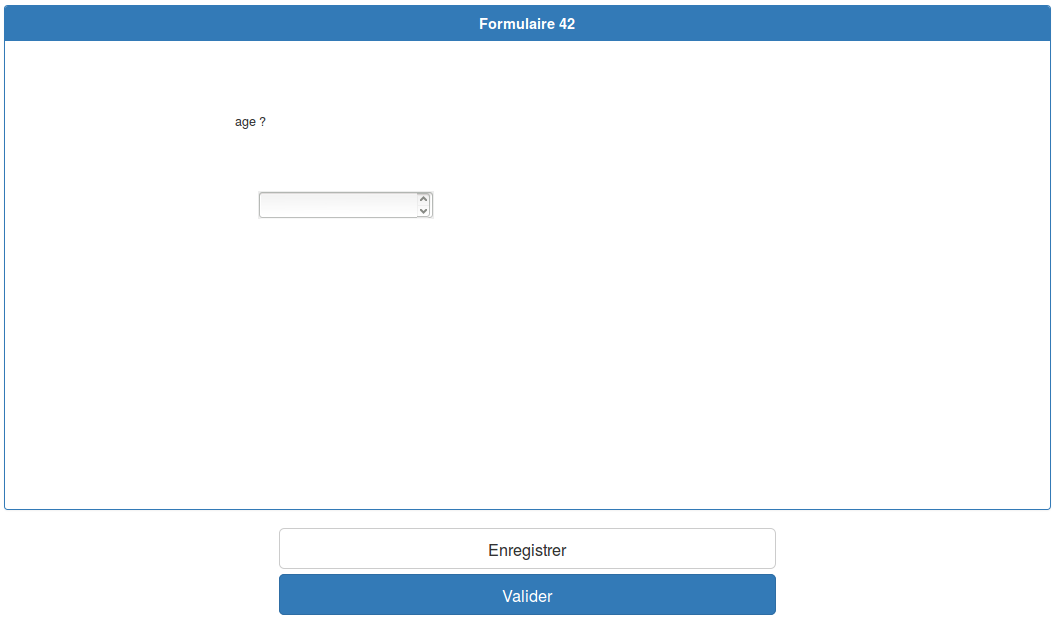
\includegraphics [width=150mm]{images/repondre.png}}
\captionof{figure}{Zone de réponse}\label{repondre}
\end{minipage}

Après avoir rempli les champs, vous avez deux possibilités, enregistrer la réponse pour la modifier plus tard ou la valider (Envoyer), dans ce cas elle ne sera plus modifiable.

\section{Modifier votre réponse}
Afin de modifer votre réponse, cliquer sur ``Réponse \#'' du formulaire souhaité sur la page figure~\ref{listRepMulti}.\\
La page de réponse figure~\ref{repondre} s'affichera pré-remplie avec vos réponses enregistrées. Modifiez ce que vous souhaitez et vous pouvez ensuite soit enregistrer soit valider votre réponse.



\chapter{FAQ}
\section{Mon écran n'affiche pas correctement la page}
Changez la résolution, zoomez ou dezoomez grâce à la combinaison Ctrl + roulette de la souris.
\section{Puis-je mettre des destinataires dont je connais l'email ?}
Non, il est nécessaire que tous les destinataires aient un compte CAS. Si vous souhaitez envoyer un formulaire à un membre exterieur, vous pouvez créer un formulaire anonyme et le lui soumettre en lui envoyer l'url du formulaire.
\section{Je ne comprends rien aux groupes, je veux juste envoyer un formulaire à une personne}
Dans ce cas, remplissez juste le(s) destinataire(s) et le nombre maximum de réponse pour ce formulaire par une même personne du groupe ``Éléments restants''. Puis créer votre formulaire normalement.
\section{Trop de réponses me reviennent}
Si trop de réponses vous reviennent c'est que vous avez fait des groupes et que le nombre de destinataires de chaque groupe multiplié entre eux et multiplié aux nombres de réponses par groupe est très élevé. Vérifiez ces informations.

\chapter{Annexe}
\section{Description des éléments}
\subsection{Label}
Si vous souhaitez placer du texte dans le formulaire, mettez un label, puis remplissez la valeur ``Value'' des paramètres par le texte désiré.
\subsection{Nombre}
Si vous souhaitez mettre un champs d'entrée que le destinataire devra remplir par un nombre, mettez un champs nombre. Vous pouvez paramétrer le nombre minimum et maximum que les destinataires seront autorisés à remplir.
\subsection{Date}
Pour un champs de date.
\subsection{Heure}
Pour un champs de heure.
\subsection{Paragraphe}
Si vous souhaitez proposer aux destinataires un champs plus large pour écrire un paragraphe.
\subsection{Input Text}
Si vous souhaitez proposer aux destinataires un champs de texte court.
\subsection{Boutons radios}
Si vous souhaitez proposer aux destinataires plusieurs choix mais qu'il ne puisse en selectionner qu'un, mettez des boutons radios. Après son placement sur la page quadrillée, un bouton ``+'' apparaitra dans la zone de paramétrage des éléments. Cliquez sur ``+'' pour pouvoir ajouter des valeurs. Cliquez sur ``-'' pour en éliminer.
\subsection{Checkbox}
Les checkbox fonctionne comme les boutons radios sauf que les destinataires pourront sélectionner plusieurs réponses au lieu d'une unique.
\subsection{Carré}
Si vous souhaitez placer un carré redimensionnable par la suite en rectangle de n'importe quelle taille.
\subsection{Cercle}
Si vous souhaitez placer un cercle redimensionnable par la suite en ovale de n'importe quelle taille.
\subsection{Image}
Si vous souhaitez insérer une image dans le formulaire, drag'n'droppez ``Image'' puis cliquez sur ``Browse'', sélectionnez enfin l'image voulu. Elle s'affichera dans le formulaire.

\end{document}
